\normaltrue \difficilefalse \tdifficilefalse
\correctionfalse

%\UPSTIidClasse{11} % 11 sup, 12 spé
%\newcommand{\UPSTIidClasse}{12}

\exer{Assemblage par frettage $\star$ \label{B2:14:Coulomb:532}}
\setcounter{numques}{0}
\UPSTIcompetence[2]{B2-14}
\index{Compétence B2-14}
\index{Lois de Coulomb}
\ifcorrection
\else
\textbf{Pas de corrigé pour cet exercice.}
\fi


\ifprof
\else

Le frettage consiste à encastrer deux pièces en utilisant le phénomène d’adhérence. 
 
Avant l’assemblage réalisé à l’aide d’une presse, l’arbre 1 
possède un diamètre légèrement supérieur à celui de l’alésage 
(trou cylindrique) de la pièce 2 dans laquelle il vient se loger. 
 
Après frettage, il subsiste donc une pression de contact $p$ 
(souvent supposée uniforme sur toute la surface de contact) 
entre les deux pièces. 

 
Les caractéristiques de cet assemblage par frettage sont les suivantes : 
\begin{itemize}
\item $R$ : rayon de l’arbre 1;
\item $L$ : longueur du contact; 
\item $f$ : facteur d’adhérence entre les deux pièces.
\end{itemize}



\begin{center}
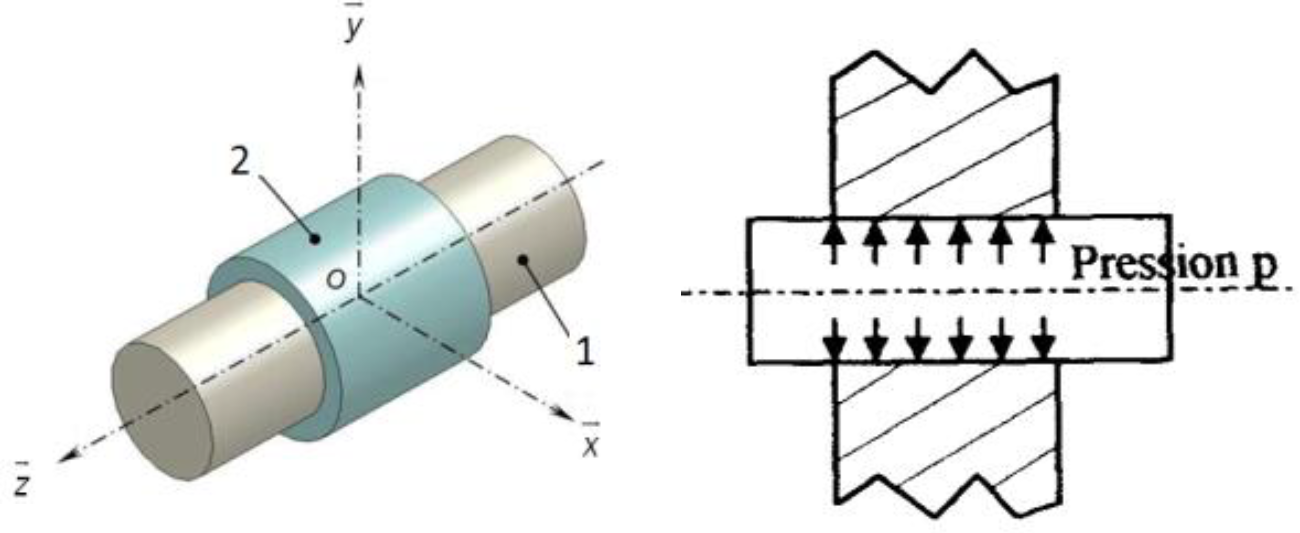
\includegraphics[width=\linewidth]{532_01}
\end{center}


\begin{obj}
Déterminer l’effort axial maximal transmissible et le couple maximal transmissible d’une pièce à 
l’autre.
\end{obj}

\subsection*{Effort axial maximal transmissible}


L’effort axial maximal transmissible correspond à la valeur maximale de la 
composante axiale de la résultante de l’action mécanique qui peut être transmise 
d’une pièce à l’autre sans qu’elles se désolidarisent. 
 
Pour simplifier notre étude, on considère la pièce 2 fixe et on cherche à déterminer 
la composante axiale de la résultante de l’action mécanique à appliquer à la pièce 1 
pour atteindre le glissement de 1/2 suivant $-\vect{z}$. 


\begin{center}
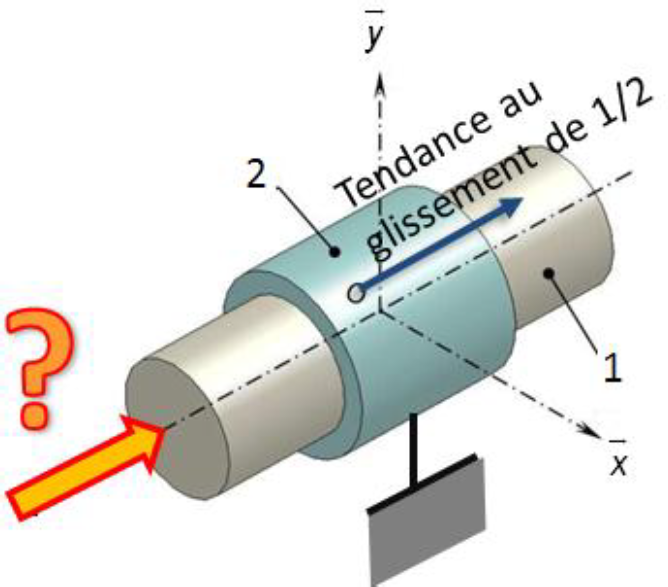
\includegraphics[width=.8\linewidth]{532_02}
\end{center}

\fi


\question{Refaire en grand les 2 schémas : un 
dans le plan $(\vect{y}, \vect{z})$ et l’autre dans le plan $(\vect{x}, \vect{y})$, 
en plaçant les actions élémentaires normale et 
tangentielle de 2 sur 1 en un point $Q$ 
quelconque de la surface de contact. }


\ifprof
\else
\begin{center}
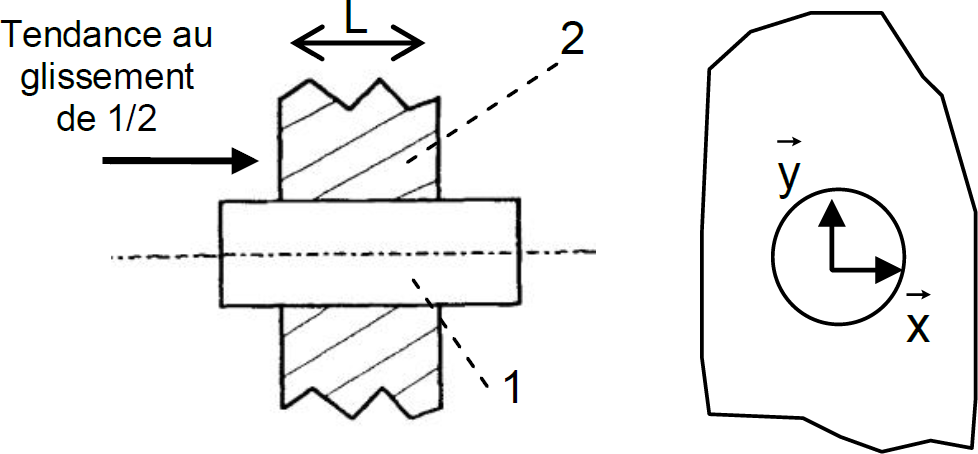
\includegraphics[width=.8\linewidth]{532_03}
\end{center}
\fi


\question{Exprimer $\vect{dF_{2\rightarrow 1}(Q)}$.}

\question{Déterminer la résultante axiale maximale transmissible en fonction de $p$ et des 
caractéristiques géométriques du frettage. }

\ifprof

Exprimons le torseur des actions mécaniques sous sa forme locale en un point $M$ : 

$$
\torseurl{d\vectf{2}{1}}{d\vectm{M}{2}{1}=\vect{0}}{M}
$$

La forme globale au point O est alors donnée par :

$$
\torseurstat{T}{2}{1} = \torseurl{\vectf{2}{1} = \int d\vectf{2}{1}}{\vectm{M}{2}{1} = \int d\vectm{M}{2}{1}= \int \vect{OM}\wedge d\vectf{2}{1}}{M}
$$

\vspace{.5cm}

\textbf{Calculons $\vectf{2}{1}$.}

$$
\vectf{2}{1} = \int d\vectf{2}{1} = \iint p \vect{-r} dS = -p \iint  \vect{r} dS
= -p \iint  \left(\cos\theta\vect{x}+\sin\theta\vect{y} \right) dS $$

$$
\vectf{2}{1}
= -p \int\limits_{-L/2}^{L/2} \int\limits_{-\pi/2}^{\pi/2}   \left(\cos\theta\vect{x}+\sin\theta\vect{y} \right) Rd\theta dz
= -p R L \int\limits_{-\pi/2}^{\pi/2}   \left(\cos\theta\vect{x}+\sin\theta\vect{y} \right) d\theta 
$$
$$
\vectf{2}{1}
= -p R L \left(\int\limits_{-\pi/2}^{\pi/2}   \cos\theta\vect{x}d\theta + \int\limits_{-\pi/2}^{\pi/2} \sin\theta\vect{y} d\theta \right)
= -p R L \left(\left[\sin\theta \right]_{-\pi/2}^{\pi/2}\vect{x}
+\left[ -\cos\theta\right]_{-\pi/2}^{\pi/2}\vect{y}
\right)
$$

$$
\vectf{2}{1}
= -p R L \left(2\vect{x}
+0\vect{y}
\right) = -2pRL\vect{x}
$$

$2RL$ est appelée surface projetée du cylindre. Elle correspond au produit du diamètre par sa longueur.

\vspace{.5cm}

\textbf{Calculons $\vectm{M}{2}{1}$.}
$$
\vectm{M}{2}{1} = \int d\vectm{M}{2}{1}= \int \vect{OM}\wedge d\vectf{2}{1}
$$

$$
\vectm{M}{2}{1} = -p \iint R\vect{r} \wedge \vect{r}dS = \vect{0}
$$

Au final, 
$$
\torseurstat{T}{2}{1} = \torseurl{\vectf{2}{1} = -2pRL\vect{x}}{\vectm{M}{2}{1} =  \vect{0}}{M}
$$

\else
\fi





\question{Calculer $\vectf{2}{1}$ lorsque la pression est de la forme : $p(\theta)=p_0\cos\theta$ pour $\theta\in[-\pi/2,\pi/2]$.}
\ifprof
Dans ce cas : 
$$
\vectf{2}{1} = \int d\vectf{2}{1} = \iint p(\theta) \vect{-r} dS 
= - p_0R\iint\cos\theta  \left(\cos\theta\vect{x}+\sin\theta\vect{y} \right)  d\theta dz$$

$$
\vectf{2}{1} 
= - p_0 L R\int\limits_{-\pi/2}^{\pi/2}\cos\theta  \left(\cos\theta\vect{x}+\sin\theta\vect{y} \right)  d\theta$$

$$
\int\limits_{-\pi/2}^{\pi/2}\cos^2\theta  d\theta = \dfrac{\pi}{2}
\quad 
\text{et}
\quad
\int\limits_{-\pi/2}^{\pi/2}\cos\theta \sin\theta  d\theta = 0
$$
Au final :
$$
\vectf{2}{1} 
= - p_0 L R \dfrac{\pi}{2}\vect{x}$$
\else
\fi



\ifprof
\else
\begin{flushright}
\footnotesize{Corrigé  voir \ref{B2:14:Coulomb:532}.}
\end{flushright}%
\fi